% !TeX spellcheck = en_US
%Publications.tex
%\newcommand{\PublicationsPath}{PatentsAndPublications/Publications}

%IEEETBC2020

\section[Predictive CDN selection for video delivery based on LSTM network performance forecasts and cost-effective trade-offs]{Predictive CDN selection for video delivery based on LSTM network performance forecasts and cost-effective trade-offs}
\label{chap:IEEETBC2020}
\begin{itemize} \itemsep1pt\parskip0pt\parsep0pt
	\item \textbf{Title:} Predictive CDN selection for video delivery based on LSTM network performance forecasts and cost-effective trade-offs
	\item \textbf{Authors:} Roberto~Viola, \'Angel~Mart\'in, Javier~Morgade, Stefano~Masneri, Mikel~Zorrilla, Pablo~Angueira and Jon~Montalb\'an
	\item \textbf{Journal:} IEEE Transactions on Broadcasting
	\item \textbf{Publisher:} IEEE
	\item \textbf{Year:} 2020
	\item \textbf{DOI:}  \url{10.1109/TBC.2020.3031724}
\end{itemize}	

\textbf{Abstract:} Owing to increasing consumption of video streams and demand for higher quality content and more advanced displays, future telecommunication networks are expected to outperform current networks in terms of key performance indicators (KPIs). Currently, content delivery networks (CDNs) are used to enhance media availability and delivery performance across the Internet in a cost-effective manner. The proliferation of CDN vendors and business models allows the content provider (CP) to use multiple CDN providers simultaneously. However, extreme concurrency dynamics can affect CDN capacity, causing performance degradation and outages, while overestimated demand affects costs. 5G standardization communities envision advanced network functions executing video analytics to enhance or boost media services. Network accelerators are required to enforce CDN resilience and efficient utilization of CDN assets. In this regard, this study investigates a cost-effective service to dynamically select the CDN for each session and video segment at the Media Server, without any modification to the video streaming pipeline being required. This service performs time series forecasts by employing a Long Short-Term Memory (LSTM) network to process real time measurements coming from connected video players. This service also ensures reliable and cost-effective content delivery through proactive selection of the CDN that fits with performance and business constraints. To this end, the proposed service predicts the number of players that can be served by each CDN at each time; then, it switches the required players between CDNs to keep the (Quality of Service) QoS rates or to reduce the CP's operational expenditure (OPEX). The proposed solution is evaluated by a real server, CDNs, and players and delivering dynamic adaptive streaming over HTTP (MPEG-DASH), where clients are notified to switch to another CDN through a standard MPEG-DASH media presentation description (MPD) update mechanism.

\textbf{Keywords:} Content Delivery Network, MPEG-DASH, Operational Expenditure, Quality of Service.


\subsection{Introduction}
\label{sec:intro}

In the last few years, the demand for video content across the Internet has constantly increased. Video streams from professional applications, such as Industrial Internet of Things (IIoT), medical equipment, connected and autonomous cars, and from domestic services such as gaming, virtual reality, augmented reality, video over IP (VoIP) sports services, and  over-the-top (OTT) platforms are flooding networks with real-time data intensive sessions.

This evolution of Internet traffic makes evident the severity of the network’s capacity to guarantee a certain quality of service (QoS) for the video applications. To prevent network flooding and to make video delivery more efficient, content delivery networks (CDNs) employ geographically distributed and cost-effective infrastructures as a service (IaaS) to enhance media availability and delivery performance across the Internet. This hierarchical system that caches and stores video streams fosters efficiency while geographical locations track human daytime life cycles, which have a close relation with local content demands.

Furthermore, the current video traffic crosses networks working on a best-effort basis where the delivery time of network packets is not guaranteed. Thus, it may cause stalls during playback on player devices, damaging the quality of experience (QoE). The popularity of video streaming services over the Internet pushed video industry-Moving Picture Experts Group (MPEG)-and standardization bodies to create new formats which enable adaptive streaming over the already existing Hypertext Transfer Protocol (HTTP) infrastructures. Thus, they allow the player devices to adapt the content representation to the specific device capabilities (resolution, codecs, etc.) and the changeable network connectivity.

Dynamic Adaptive Streaming over HTTP (MPEG-DASH) \cite{sodagar2011mpeg}, which was designed to mitigate problems due to fluctuations on best-effort networks, is the solution adopted by the video industry \cite{park2017}. In fact, MPEG-DASH enables pull-based streaming \cite{begen2011} and allows for scalable distribution as it has a CDN-ready design \cite{maille2016} that enables the exploitation of existing HTTP caching infrastructures without modifications. To this end, the MPEG-DASH pipeline splits the video content into segments of fixed duration, usually between 2 and 10 seconds; then, it encodes them at different representation levels with a nominal resolution and bitrate. Thus, for each segment request, the player can switch from one representation to another depending on the assessed network status.

Nevertheless, the MPEG-DASH client-driven approach presents some drawbacks. First, each player is not aware of the existence of the others, leading to high network dynamics as the content download is not coordinated. Second, each player strives to achieve optimized individual quality, which may lead to unfairness when a congested connection path is shared \cite{akhshabi2012}. Thus, it is challenging for a content provider (CP) to ensure a certain level of quality to end users, who are accessing large volumes of content through the same access point and competing for the available bandwidth independently. Here, some issues, such as initial buffering delay, temporal interruptions, unsteady video resolution, and bitrate changes, may damage the QoE \cite{Seufert2014}.

Currently, CDNs are used to enhance media availability and delivery performance across the Internet. The proliferation of CDN vendors and business models allows the CP to use multiple CDN providers simultaneously \cite{adhikari2012}, \cite{adhikari2012-2}, \cite{adhikari2015}. However, extreme concurrency dynamics can affect CDN capacity, causing performance degradation and outages, while overestimated demand affects costs, thereby increasing the operational expenditure (OPEX) of the CP \cite{silva2020}.

Upcoming 5G networks will need advanced and intelligent mechanisms to dynamically deliver each data flow according to the required service level agreement (SLA) and considering performance costs trade-offs.
This concept is where the approach proposed by this paper takes place, fusing network characteristics and media service options to match user satisfaction and business policies.

\subsubsection{Contribution}
\label{sec:overview}

This work proposes a novel solution called intelligent network flow (INFLOW) for CDN selection in a multi-CDN delivery environment. It exploits periodical MPEG-DASH media presentation description (MPD) updates to apply dynamic switching among the available CDNs at the video players in a standard compliant manner. The MPD with the appropriate CDN endpoint is served by the INFLOW Media Server, which works jointly with the INFLOW Forecast Service. The INFLOW Forecast Service provides network metrics predictions based on a Long Short-Term Memory (LSTM) network, a kind of Recurrent Neural Network (RNN), when fed with the historical values of network metrics. The integration of the Forecast Server into the delivery chain allows the Media Server to serve an MPD containing the \textit{BaseURL} of the CDN, which fits target QoS and CP's business requirements. Thus, INFLOW allows for proactive and cost-effective video streaming delivery. 
The proposed solution comprises the following relevant contributions:
\begin{itemize}
	\item Exploitation of network performance metrics and MPD information to apply common decisions to ongoing streaming sessions. Captured network metrics are employed to forecast CDN server capacity, then select a CDN only if it would guarantee the viability to serve the content at a minimum representation bitrate from the available ones in the MPD.
	\item Dynamic CDN server switching. We employ a dynamic approach switching from a CDN server to another depending on the performed predictions at any time. Thus, in contrast to current solutions, a streaming session is not served from a single CDN provider.
	\item Practical application of a forecast model. The literature proposing a forecast model for QoS network metrics is usually limited to theoretical analysis and simulations, and the predictions are not turned into video streaming actions. On the contrary, we exploit the predictions to switch the players among the available CDN servers, then proactively act on the delivery.
	\item Business constraints are considered for the CDN selection. We include metrics for both the OPEX and the QoS in the algorithm which selects the ideal CDN to be employed. Thus, this sophisticated approach favours the dynamic utilisation of a CDN marketplace to deal with cost-effective trade-offs. OPEX reduction, while keeping the QoS, is a major concern for practical deployments in real-world streaming services.
\end{itemize}
To achieve the above contributions, we develop a Forecast Service and a Media Server as complementary parts of the proposed INFLOW solution. Forecast Service executes an LSTM network performing real-time predictions of the QoS metrics. Media Server updates the MPD according to the network metrics predictions and CP's business rules and serves it to the clients.
The solution was integrated and tested in a real setup employing a multi-modal testbed including both wired and wireless nodes. The wireless nodes were connected through a real Long-Term Evolution (LTE) RAN infrastructure of an operational Mobile Network stack including the radio base station (eNodeB) and the Evolved Packet Core (EPC). The traffic demand on video players was generated according to a probability distribution widely employed in the literature.

The paper is structured as follows. First, section \ref{sec:sota} reviews related work in the field of video delivery based on CDN performance and network traffic generation and forecast. Then, section \ref{sec:system} introduces the proposed INFLOW server, a novel media server equipped with a forecast service that tunes the delivery and applies a CDN selection mechanism based on QoS metrics and business rules, as the main focus of the article. Section \ref{sec:setup} describes the implemented setup using a real testbed, while section \ref{sec:validation} presents the results of the validation experiments. Finally, we assert our conclusions and future work in section \ref{sec:conclusion}.


\subsection{Related Work}
\label{sec:sota}

\textbf{\subsubsection{CDN resource selection}
	\label{sec:cdnselection}}

A CDN is a network function widely employed to improve content delivery by means of cloud service provisioning cache features. Fueled by the CDN vendor proliferation, media platforms exploit multi-CDN strategies to obtain more reliable content delivery that provides a steadier QoS and higher customer satisfaction. Nevertheless, the CDN selection criteria can be different for any CP.

A widely employed solution applies a static selection made by the media server when a new streaming session starts. This is used by Netflix \cite{adhikari2012} and Hulu \cite{adhikari2012-2}, with big similarities \cite{adhikari2015}. They use three different CDN vendors mapping CDNs to the location of client device or to a subscriber. Moreover, they evidence that, the selected CDN is fixed during the streaming session even when the QoS degrades. Thus, providers are more prone to lower the representation bitrate instead of operating alternative CDNs. Hence, the authors conjecture that CDN selection is most likely based on business policies.

However, Netflix has changed its strategy over the years, and nowadays it uses its own CDN, which is called Open Connect \cite{botteger2018}. Open Connect can be run inside the ISP infrastructure so that a better QoS can be achieved as the content is closer to the user. Netflix’ solution is not that different from the open CDN architecture proposed by \cite{zhang2014}. The authors propose collaborative participation of CPs and ISPs. On one hand, cost reductions are realized as the ISP acts as a CDN. On the other hand, the ISP provides better performance to the clients and reduces traffic as the content is already present in its network infrastructure.

The awareness of end-to-end QoS metrics measured by the client can make the difference when the employed CDN is dynamically chosen by the clients. The authors of \cite{otto2012} propose a client-side CDN selection. As a drawback, client-side strategies do not produce a coordinated decision as each client analyses the network performance of each CDN independently, introducing bias and communication overheads. Hence, a client-side CDN selection is not an optimal solution.

An intermediate solution consists of Domain Name System (DNS) resolution. Here, the DNS server can resolve a fixed hostname owned by the CP into different IP addresses of several CDNs. Depending on the DNS resolution, the client is directed to an appropriate CDN. The YouTube DNS-based solution is shown in \cite{torres2011}. YouTube goes further as it allows for the use of a hybrid DNS and application-level CDN selection. First, the DNS redirects the client to a server. Then, the server accepts or reject the client depending on the workload. If the client is refused, the DNS redirects the client to another server.

In \cite{goel2015}, the effects of DNS resolution for CDN selection are further studied. The authors conclude that, depending on the DNS service provider, Akamai and Google CDN servers are chosen differently. Consequently, CDN performance highly depends on the load balancing rules of the DNS server. Here, a suboptimal CDN server selection leads to a higher round-trip delay time (RTT). To solve this problem, the authors propose a DNS-proxy running on the client. This proxy forwards the DNS requests to different DNS servers; then, it compares the responses to identify the best performing CDN server. However, these solutions are loosely coupled from media player requests slots applying balancing policies independently of media player timing. Instead, out approach is triggered by the requests with the most recent available information.

CDN Brokering \cite{biliris2002} is the ability to redirect clients dynamically among two or more CDNs. CDN brokers collect and analyze the performance metrics of the available CDNs to select the one that performs best. Their work, in contrast to traditional multi-CDN strategies, is not limited to the selection of the initial CDN for each client. This solution also moves clients between CDNs when performance degradation is detected in real time. Thus, the CDN is dynamically and seamlessly changed. As an example, the European Broadcasting Union (EBU) proposed the EBU Flow Multi-CDN \cite{EurovisionFLOW}, which consists of a CDN switching service that selects the optimal CDN at any time. Similar approaches are provided by Citrix \cite{citrix2} and LightFlow \cite{lightflow}. Thus, these solutions are usually provided by intermediaries, federating infrastructures from different vendors. However, our approach keeps the control to the media service manager able to dynamically change the business policy or tune the cost function.

Edge computing systems promise a revolution on smart delivery of media traffic fueled by Multi-access Edge Computing (MEC) \cite{etsi2019} architectures from 5G.
Thus, new solutions for improving multi-CDN delivery involve investigating MEC services. In \cite{viola2018} a MEC proxy is proposed. The proxy can retrieve video streaming metrics of video players at the access point transparently and CDNs performance metrics from the wired link. Compared to a pure client-decision, a MEC proxy can evaluate the performance of each CDN just once and apply conclusions to other sessions (independently from the number of connected players). Moreover, it empowers the delivery through a local edge cache. This feature guarantees traffic reduction compared to server-side CDN selection as recurrent content can be downloaded and cached once for every client. In \cite{carrozzo2018}, a similar solution for a MEC-based cache is proposed.
However, till the moment the edge systems realize, current CDN infrastructures makes the difference, and universal solutions that dynamically manage balancing are required.

In \cite{frank2013}, a prototype of CDN and ISP collaboration is proposed. The ISP provides the CDN provider with services that allow the CDN provider to retrieve geographical user distribution and allocate server resources inside the ISP's network topology. The authors of \cite{wichtlhuber2015} propose a similar solution without the binding to allocate resources in the ISP's infrastructure. In this case, a redirection center inside the ISP's network intercepts the client’s requests and selects the appropriate CDN. This process is transparent to the client as the redirection center stores the content in a CDN surrogate and instructs an OpenFlow controller to migrate the traffic to a CDN surrogate.

Contrary to those approaches provisioning or balancing serving resources, other works focus on the selection of the appropriate bitrate to avoid congestion for a static number of servers \cite{sadi2020} or network assets \cite{giannone2020}. To this end, the MPD is parsed and heavier options are cropped. As implemented in these works, our approach employs a compliant MPD update mechanism. But, in our case, it is exploited to dynamically manage the CDN resources at any moment depending on network performance forecasts and CP business rules. The CP can tune the media server, thereby influencing CDN selection when the video player requests an MPD update.

\subsubsection{Time series for network traffic forecast}
\label{sec:timeseries}

\begin{table}[t]
	\caption{Forecast models comparison}
	\centering
	\label{tab:IEEETBC2020models}
	\def\arraystretch{1.2}%  1 is the default, change whatever you need
	\setlength\tabcolsep{2.0pt} % default value: 6pt
	{\scriptsize
	\begin{tabular}{>{\centering\arraybackslash}m{\dimexpr0.2\textwidth-2\tabcolsep-\arrayrulewidth\relax}
			>{\centering\arraybackslash}m{\dimexpr0.15\textwidth-2\tabcolsep-\arrayrulewidth\relax}
			>{\centering\arraybackslash}m{\dimexpr0.15\textwidth-2\tabcolsep-\arrayrulewidth\relax}
			>{\centering\arraybackslash}m{\dimexpr0.5\textwidth-2\tabcolsep-\arrayrulewidth\relax}
		}
		\toprule
		\textbf{Model} & \textbf{Approach} & \textbf{Number of variables} & \textbf{Internal parameters}\\
		\midrule
		\midrule
		ARIMA & statistical & univariate & a-priori (regression, integration and moving average parameters)\\
		Exponential smoothing & statistical & univariate & a-priori (smoothing factor)\\
		SETARMA & statistical & univariate & a-priori (regression, moving average and threshold delay parameters)\\
		GARCH & statistical & univariate & a-priori (regression and lag length parameters)\\
		Feed-forward NN & neural network & multivariate & trained (weight and bias)\\
		RNN & neural network & multivariate & trained (input, output and forget factors)\\
		LSTM & neural network & multivariate & trained (input, output and forget factors)\\
		\bottomrule
		\bottomrule
	\end{tabular}
	}
\end{table}

The goal of applying time series analysis to network traffic data is to forecast future conditions to take actions proactively when actuation performance or cost policies are satisfied. These techniques allow network management systems to prevent network under-performance and outages, thereby addressing network congestion preemptively.

The auto-regressive integrated moving average (ARIMA) is employed in \cite{calheiros2014} to predict the workload of cloud services. It employs historical records of observed requests to predict the volume of requests for the following time interval. The results reveal that the model can obtain the general trend, but it lacks the ability to accurately and timely track traffic peaks. The authors of \cite{dong2015} apply both ARIMA and exponential smoothing models to predict throughput in an LTE network. The two models are complementary, with ARIMA outperforming the exponential smoothing models on weekdays and the exponential smoothing models outperforming ARIMA on weekends.

The authors of \cite{amin2012} and \cite{amin2012-2} found limitations in ARIMA while modelling QoS attributes. QoS attributes such as bandwidth or latency have nonlinear behaviors that do not fit the linear assumption of the ARIMA model. They overcame this by introducing hybrid linear and non-linear models. The linear model was represented by the ARIMA model. For the non-linear model, \cite{amin2012} used the self-exciting threshold autoregressive moving average (SETARMA) model, while \cite{amin2012-2} employed a generalized autoregressive conditional heteroscedastic (GARCH) model. In both cases, the proposed solution outperforms a standalone ARIMA model in forecasting the time between QoS violations.

In recent years, machine learning (ML)-based techniques for time series prediction have exhibited satisfactory performances. Specifically, neural networks (NNs) are gaining adoption in the generation of time series models. The authors of \cite{zadeh2010} propose a feed-forward NN for predicting the execution time of services while varying the number of requesters. In \cite{belhaj2009}, a recurrent NN (RNN) is employed to forecast the end-to-end delay from RTT metrics.

In \cite{trinh2018}, an LSTM model, a particular type of RNN, was proposed. The authors employed a multivariate time series model where data input was probed from downlink control information (DCI) messages, such as resource blocks, transport block size, and scheduling information.

Table \ref{tab:IEEETBC2020models} shows the main differences between the employed techniques for time series forecasting. Clearly, NN-based approaches have the advantage to employ several variables as input and/or output of the models, while statistical ones are limited to one. Moreover, statistical approaches need a-priori evaluation of internal parameters, while NN-based ones are trained through a dataset of previous collected metrics. Here, the parameters for statistical approaches are intended for the whole model, while for NN-based ones, parameters must be trained for each internal cell.

From the available algorithms to analyze and predict time series, we employ LSTM network model as it satisfies two requirements. First, in terms of accuracy, statistical solutions (ARIMA and its derivatives) are slow when tracking quick fluctuations in time series as they tend to concentrate on the average value of the past observed values, as revealed in \cite{wang2017}. Second, in terms of multivariate time series, statistical solutions only can predict one variable. Thus, ARIMA would require separate models for forecasting both latency and bandwidth. On the contrary, LSTM is ready to process multivariate time series. The authors of \cite{azari2019} and \cite{azari2019-2} revealed that, the higher the number of input variables, the better the traffic predictions of LSTM when compared to ARIMA.

% needed in second column of first page if using \IEEEpubid
%\IEEEpubidadjcol

\subsection{INFLOW solution}
\label{sec:system}

\subsubsection{System architecture}
\label{sec:detailedcontribution}

To achieve reliable and cost-effective video delivery, we propose the inclusion of our INFLOW solution in the video delivery chain. The overall scenario of the solution is depicted in Figure \ref{fig:IEEETBC2020scenario}. The INFLOW solution is composed of two components:
\begin{itemize}
	\item INFLOW Forecast Service: it receives the QoS performance metrics from the video players and processes them to predict the QoS values in the future.
	\item INFLOW Media Server: it exploits the results provided by the Forecast Service by combining them with the CP's business rules to select the appropriate CDN for each client.
\end{itemize}

\begin{figure}[htp]
	\centering
	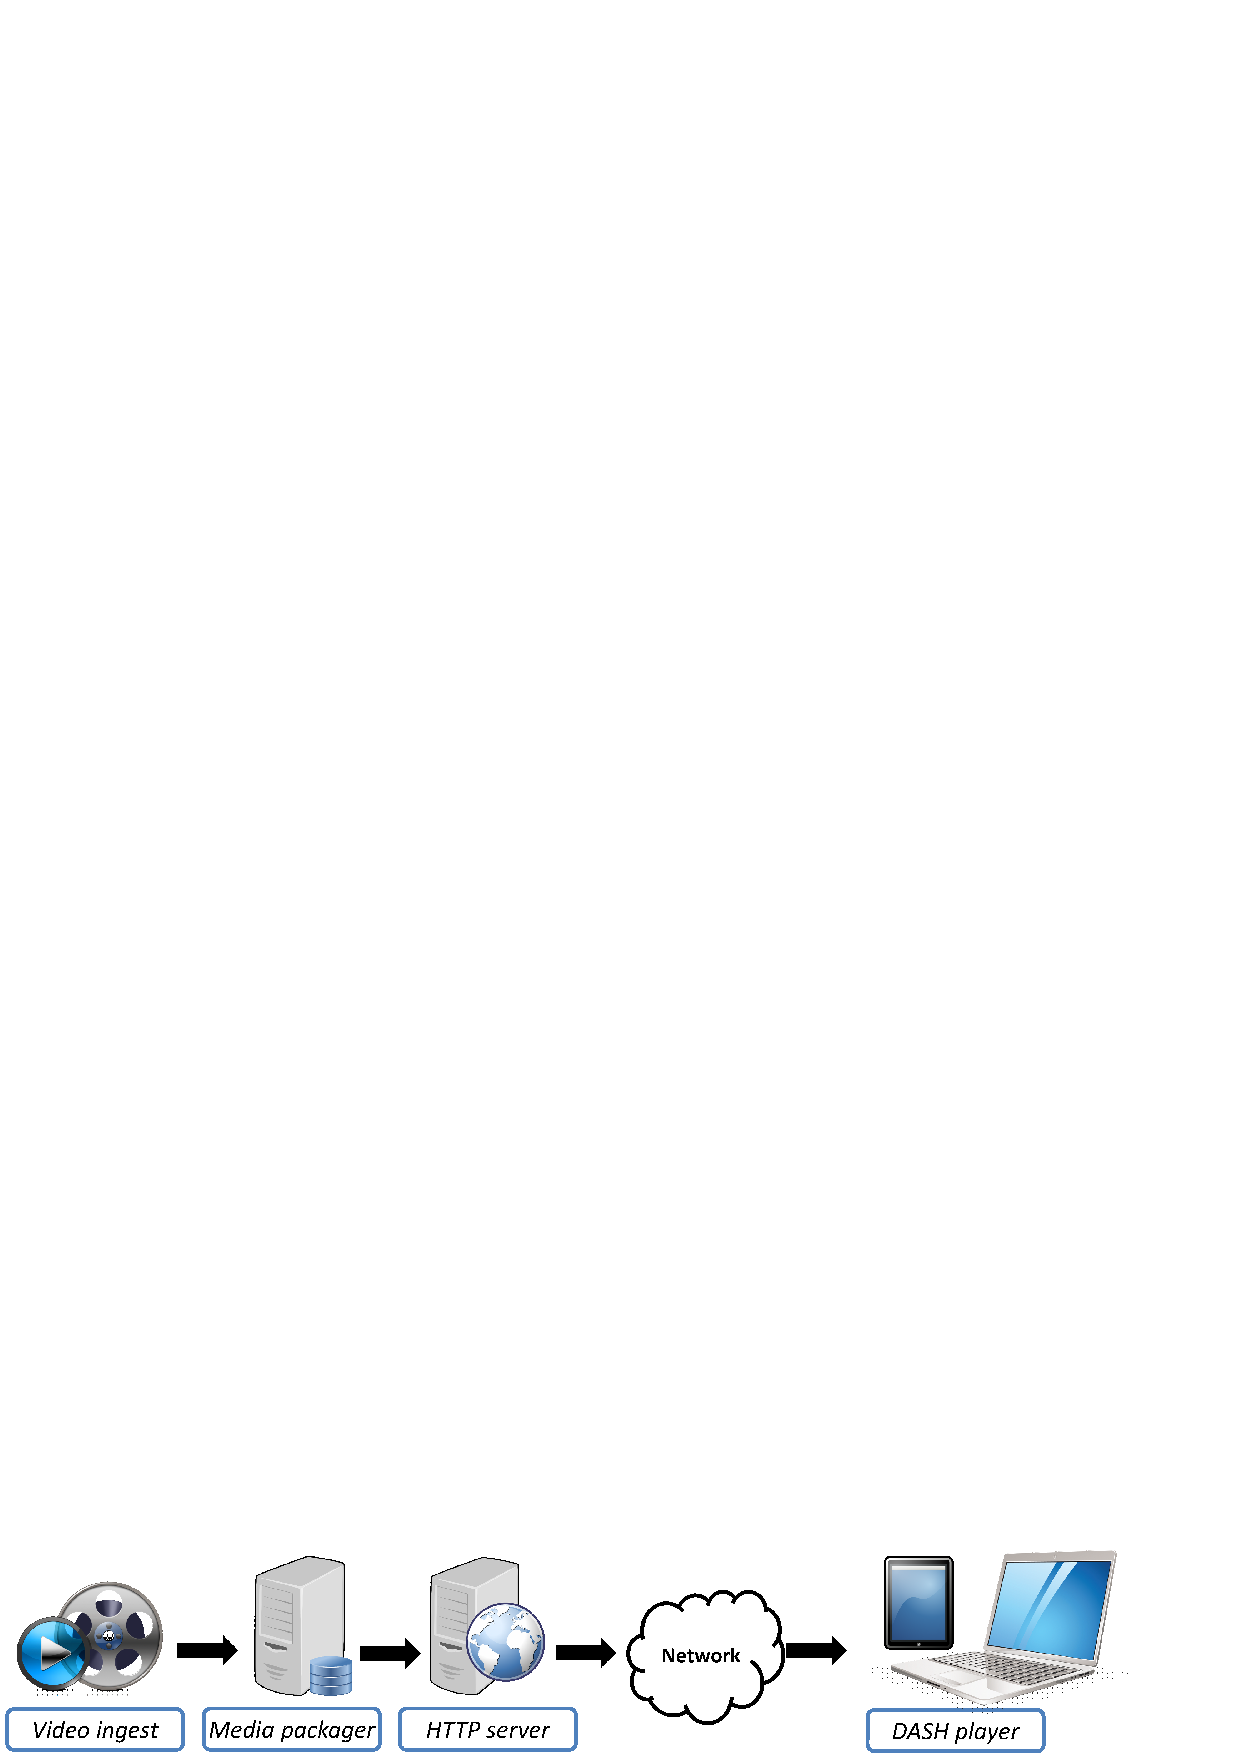
\includegraphics[width=1\textwidth,keepaspectratio]{system.pdf}
	\caption{General scenario of the proposed solution.}
	\label{fig:IEEETBC2020scenario}
\end{figure}

Owing to the utilization of MPEG-DASH, INFLOW includes the following features:
\begin{itemize}
	\item Scalability. New CDNs can be easily managed by adding them to the initial MPD.
	\item Real-time migration of video players to CDN providers. Supported by standard-compliant MPEG-DASH MPD update mechanism manages the utilization of a CDN by the video player according to the gathered metrics and business policies.
	\item MPDs can be parsed and processed even when the content is encrypted with the MPEG-DASH Common Encryption Scheme (CENC) \cite{isocenc}. The CENC format encrypts the media segments indexed in the MPD, but the MPD is not encrypted.
\end{itemize}

The sequence diagram of the exchanged messages is depicted in Figure \ref{fig:IEEETBC2020seqdiag2}. Media segments are stored at different CDNs, while the MPD is served by the INFLOW Media Server. It is important that the media server uses a dynamic MPD as it forces the player to periodically update, overwriting the Minimum Update Period attribute from the MPEG-DASH standard \cite{lohmar2011}. On the other side, each video player downloads the initial MPD and starts requesting for segments from the initial CDN. A client-side adaptation mechanism constantly monitors the statistics of the downloaded segments to select a representation level among those available that fits with the experienced network performance. Thus, the video player aims to prevent stalls during playback. Typical monitored metrics are the network bandwidth and latency, which provide a direct measure of the QoS experienced by the client. Moreover, these measurements are sent to the INFLOW forecast service. Thus, video player should support a mechanism for sending feedback to the forecast service, such as Server and Network-assisted DASH (SAND) standard \cite{thomas2016}. Finally, INFLOW forecast service stores the measurements and uses them to predict the future values.

\begin{figure}[htp]
	\centering
	\includegraphics[width=0.65\textwidth,keepaspectratio]{communication.png}
	\caption{Sequence diagram of the INFLOW solution for video delivery.}
	\label{fig:IEEETBC2020seqdiag2}
\end{figure}

The MPD served by the media server is fully conditioned by the prediction of the forecast service. Every time a player requests an updated version of the MPD, the media server retrieves a prediction from the forecast service and decides to serve the current MPD or to change the CDN included. Therefore, the forecast service does not apply any QoS or business rules—it simply processes the information provided by the players. The QoS and business-based decisions are made by the media server, and this decision process is executed in real-time as the predictions are rendered out of date after the predicted interval, leading to a new decision. Therefore, the shorter is the segment duration, the more immediate is the forecast validity and the prompter is the MPD update.

The QoS forecasts serve two roles. First, the INFLOW Media Server can select an appropriate CDN to shield from CDN service degradation and outages based on the most recent detected performance. To this end, the server receives alternative CDNs from the initial MPD and replaces the \textit{BaseURL} tag in the MPD with another CDN endpoint to migrate a client. Second, the media server can count the video sessions served by each CDN. On top of this information, the media server can apply cost-effective policies, allocating extra CDN resources to enforce QoS or retiring CDN assets to reduce the number of employed CDN servers. Thus, the media service can manipulate the OPEX ranges to meet the business model.

In the following section, we describe separately the two components of the INFLOW solution.

\subsubsection{INFLOW Forecast Service}
\label{sec:forecastservice}

The INFLOW forecast service is in charge of collecting network metrics probed and sent by the video players and processing them to predict the values in future slots. The most recent metrics are processed while older ones are discarded using a sliding window mechanism. The decision program of the forecast service is shown in Algorithm \ref{alg:IEEETBC2020algorithmForecast}.

\begin{algorithm}
	\renewcommand{\algorithmicrequire}{\textbf{Input:}}
	\renewcommand{\algorithmicensure}{\textbf{Output:}}
	\caption{INFLOW Forecast Service}
	\label{alg:IEEETBC2020algorithmForecast}
	\begin{algorithmic}
		\Function{predictMetrics}{$\overline{bw_{t-1}^{k}}$, $\overline{l_{t-1}^{k}}$, $CDN^{k}$}
		\State \Comment{for each CDN infrastructure}
		\Require $\overline{bw_{t-1}^{k}}$ \Comment{\parbox[t]{.5\linewidth}{bandwidth mean for the \linebreak most recent period @$CDN^{k}$}}
		\Require $\overline{l_{t-1}^{k}}$ \Comment{\parbox[t]{.5\linewidth}{latency mean for the \linebreak most recent period @$CDN^{k}$}}
		\Ensure $\widehat{{bw}_{t}^{k}}$ \Comment{bandwidth prediction}
		\Ensure $\widehat{{l}_{t}^{k}}$ \Comment{latency prediction}
		\State $\{bw^{k}\}$ = \{$\overline{bw_{t-1}^{k}}$,...,$\overline{bw_{t-N}^{k}}$\} \Comment{N bandwidth samples}
		\State $\{l^{k}\}$ = \{$\overline{l_{t-1}^{k}}$,...,$\overline{l_{t-N}^{k}}$\} \Comment{N latency samples}
		\State $\widehat{{bw}_{t}^{k}}$,$\widehat{{l}_{t}^{k}}$ $\leftarrow$ LSTM(\{$bw^{k}$\},\{$l^{k}$\}) \Comment{\parbox[t]{.28\linewidth}{update forecast model $CDN^{k}$}}
		\EndFunction
	\end{algorithmic}
\end{algorithm}

The input are the last \textit{N} historical values of network bandwidth and latency measured and reported by the players for a specific CDN ($CDN^{k}$). The samples comprised in the most recent period are captured during last segment download. The video player requests segments in a regular pace to fill its buffer, according to the media duration of the segment. In total, the algorithm processes two variables taken in \textit{N} time instants. Every new sample should be taken at a fixed temporal distance from the previous one. Nevertheless, this assumption of equal distance among the samples is not guaranteed as players usually run asynchronously, and then the reports are sent in a random time inside a segment slot. To overcome this problem, the INFLOW forecast server employs a mean value of samples within a second as the input of the algorithm (\{$\overline{bw_{t-1}^{k}}$,...,$\overline{bw_{t-N}^{k}}$\} and \{$\overline{l_{t-1}^{k}}$,...,$\overline{l_{t-N}^{k}}$\}). The input is processed through the LSTM network to predict the values in the next second ($\widehat{{bw}_{t}^{k}}$ and $\widehat{{l}_{t}^{k}}$). The predicted values are the output of the algorithm.

It is important to underline that the benefits of an LSTM network over statistical approaches are two-fold. First, the LSTM network performs better when time series includes quick fluctuations \cite{wang2017}. Second, it is valid for multivariate time series, such as bandwidth and latency, where statistical methods fail to simultaneously process several components \cite{azari2019}, \cite{azari2019-2}.

\subsubsection{INFLOW Media Server}
\label{sec:mediaserver}

The media server must serve the MPD of the video players to provide awareness on available representations, content formats and metadata, and CDN endpoints. In our case, as we were interested in CDN localization, the served MPD could include one or more \textit{BaseURL} tags containing the URLs of the CDN servers. In cases with only one \textit{BaseURL}, the client is forced to use it.

The INFLOW media server stores an initial MPD containing different \textit{BaseURL} tags and modifies it while excluding CDN alternatives to force a CDN to perform according to the algorithm outcomes, which exploits the predictions provided by the INFLOW forecast service. The decision program of the media server is shown in Algorithm \ref{alg:IEEETBC2020algorithmServer}.

\begin{algorithm}
	\renewcommand{\algorithmicrequire}{\textbf{Input:}}
	\renewcommand{\algorithmicensure}{\textbf{Output:}}
	\caption{INFLOW Media Server}
	\label{alg:IEEETBC2020algorithmServer}
	\begin{algorithmic}
		\Function{updateMPD}{$urlMPD$, $SLA$}
		\State \Comment{for each MPD request}
		\Require $urlMPD$ \Comment{requested MPD}
		\Require $SLA$ \Comment{applicable SLA}
		\Ensure $MPD$ \Comment{updated MPD}
		\State $MPD$ $\leftarrow$ initial($urlMPD$) \Comment{requested MPD file}
		\State $bw_{min}$ $\leftarrow$ targetQoS($SLA$) \Comment{\parbox[t]{.35\linewidth}{minimum bandwidth per player}}
		\State $d_{s}$ $\leftarrow$ $MPD$ \Comment{segment duration}
		\State \{$CDN_{list}$\} $\leftarrow$ $MPD$ \Comment{set of alternative CDNs}
		\ForAll { ${CDN}^{k}$ $\in$ \{$CDN_{list}$\} } \Comment{for each CDN}
		\State $\overline{bw_{t-1}^{k}}$ $\leftarrow$ mean(\{$bw_{[t-1,t)}^{k}$\}) \Comment{\parbox[t]{.33\linewidth}{average for most recent period @ $CDN^{k}$}}
		\State $\overline{l_{t-1}^{k}}$ $\leftarrow$ mean(\{$l_{[t-1,t)}^{k}$\})  \Comment{\parbox[t]{.33\linewidth}{average for most recent period @ $CDN^{k}$}}
		\State {$\widehat{{bw}_{t}^{k}}$,$\widehat{{l}_{t}^{k}}$} $\leftarrow$ predictMetrics($\overline{bw_{t-1}^{k}}$,$\overline{l_{t-1}^{k}}$,$CDN^{k}$)
		\State $n^{k}$ $\leftarrow$ sessions($CDN^{k}$) \Comment{total $CDN^{k}$ sessions}
		\State $\widehat{n^{k}}$ $\leftarrow$ policy($\widehat{{bw}_{t}^{k}}$,$\widehat{{l}_{t}^{k}}$,$n^{k}$,$bw_{min}$,$d_{s}$,$CDN^{k}$)
		\State \Comment{$CDN^{k}$ capacity}
		\If {($\widehat{n^{k}}$ $>$ $n^{k}$)} \Comment{$CDN^{k}$ admits more sessions}
		\State $BaseURL$ $\leftarrow$ URL($CDN^{k}$)
		\State \Comment{write $CDN^{k}$ URL}
		\State $MPD$ $\leftarrow$ update($MPD$,$BaseURL$)
		\State \Comment{update MPD}
		\EndIf
		\EndFor
		\EndFunction
	\end{algorithmic}
\end{algorithm}

The algorithm takes an initial configuration of minimum bandwidth to be provided to the clients ($bw_{min}$) according to the SLA, and the initial MPD. From the MPD, it retrieves the segment duration ($d_{s}$) and a list of the CDNs (\{$CDN_{list}$\}). When an MPD request reaches the media server, it selects an appropriate CDN ($CDN^{k}$) from the CDN list. This list (\{$CDN_{list}$\}) is ordered in ascending order according to expenses. Thus, the media server first employs the affordable providers, migrating users to cheaper services when possible. The media server retrieves the prediction for each CDN from the forecast service ($\widehat{{bw}_{t}^{k}}$ and $\widehat{{l}_{t}^{k}}$) and stops if the expected capacity ($\widehat{n^{k}}$) is higher than the current ones ($n^{k}$). In other words, it selects the most affordable CDN that has the capacity to serve more players. The number of expected players is evaluated through the predictions and the initial configuration by means of Equation \ref{eq:IEEETBC2020players}.

\begin{equation}
\label{eq:IEEETBC2020players}
\widehat{n^{k}} = \frac{(d_{s}-\widehat{{l}_{t}^{k}})*\widehat{{bw}_{t}^{k}}*n^{k}}{d_{s}*bw_{min}}
\end{equation}

To be timely delivered, the theoretical maximum download time of a segment should be lower than the segment duration. Furthermore, a padding time must be considered to take into account the delay introduced by the network during the transmission. Consequently, the predicted latency ($\widehat{{l}_{t}^{k}}$) is used as a penalization factor to estimate the effective download time ($d_{s}$-$\widehat{{l}_{t}^{k}}$). Then, this value is multiplied by the predicted average bandwidth per video player ($\widehat{{bw}_{t}^{k}}$) to assess the average volume of data that each player can download. The total data capacity is obtained by multiplying the number of sessions in the CDN ($n^{k}$) by the average volume of data that each player can download. Finally, the overall traffic demand is divided by the amount of data that a player should download during a segment duration ($d_{s}$) according to the SLA using the minimum bandwidth provided ($bw_{min}$). The final value is the CDN capacity according to an SLA, which is indicative of the number of video streaming sessions that the CDN can serve ($\widehat{n^{k}}$).

Once a CDN is assigned to a session, the media server selects the \textit{BaseURL} corresponding to the CDN and generates a new MPD by modifying the initial one. The order of the CDNs in the list is important as they are ranked depending on the cost. Thus, the media server chooses the first CDN that fits with the necessary resources; then, the most affordable ones are quickly booked to reduce CP's OPEX.

\subsection{Testbed setup}
\label{sec:setup}

To demonstrate the cost-effective advantages of the INFLOW approach in terms of QoS enforcement and CP's OPEX reduction, we deployed a heterogeneous and distributed setup employing both FED4FIRE+ facilities \cite{nussbaum2019} and our facilities at Vicomtech (San Sebastián, Spain). Fed4FIRE+ is a Horizon 2020 project that provides open and accessible testbeds to support research and innovation initiatives in Europe. Among the available facilities, we employed NITOS's network infrastructure \cite{makris2015} at University of Thessaly's campus (Volos, Greece). NITOS provides heterogeneous testbeds to execute experiments on real wired and wireless networks.

We use D-DASH dataset and infrastructure \cite{lederer2013}, with Dynamic Adaptive Streaming over HTTP (DASH) standard content mirrored over different sites at different locations to perform CDN-based scientific evaluations.
The dataset includes the Red Bull Playstreet video sequence, which is owned by Red Bull Media House and licensed for scientific purposes. This sequence is encoded for 17 video representations through advanced video coding (H.264/AVC) and 4 dual channel audio representations through advanced audio coding (AAC). Both audio and video are segmented with different segment lengths of 2, 4, 6, 10, and 15 seconds, and multiplexed in ISO MPEG4 files (ISO/IEC 14496-12 - MPEG-4 Part 12). For our experiments, we employed 2 seconds segments to focus on live video content where dense client cells and congestion of CDNs were likely. We did not modify the video representations; instead, we used the available representations in the dataset. The representations range from a resolution of 320 x 240 and 30 fps at 100 kbps to a resolution of 1920 x 1080 and 30 fps at 6000 kbps. As the client-side bitrate adaptation mechanism works on a best-effort basis and do not take care of the presence of other connected players, each player struggles to achieve the highest representation bitrate.

The final experimental setup comprises the following:
\begin{itemize}
	\item 4 UE nodes: client nodes located at NITOS and running 100 DASH video players based on GStreamer multimedia framework \cite{gstreamer}. They feature both Ethernet and LTE interfaces and are placed in the isolated environment of the NITOS indoor testbed where they form a grid topology.
	\item 1 eNodeB: USRP provided node performing eNodeB stack located at NITOS. It forwards the packets from the clients to the Access and Core Network.
	\item 1 EPC node: wired node close to the eNodeB that executes the EPC stack.
	\item 1 INFLOW Media Server: node at Vicomtech based on a virtual machine with 2 GB RAM and single-core CPU. It is provided with a public IP address to serve the MPD to the video players. It runs a Node.js \cite{nodejs} server application which applies QoS and CP's business rules when sending the MPD to the client.
	\item 1 INFLOW Forecast Service: node at Vicomtech based on a physical machine having 12 GB RAM and quad-core Intel i5 6500 CPU. To perform predictions, it features NVIDIA GTX 1050 TI executing the LSTM model based on TensorFlow \cite{tensorflow}.
	\item 3 servers: they belong to the D-DASH dataset \cite{lederer2013} providing alternative CDNs storing the media segments to perform CDN-based scientific evaluations. They are located at different sites with different nominal performances in terms of bandwidth and latency.
\end{itemize}

To distribute the video streaming sessions between the wired and LTE network interfaces, we considered the last Cisco report concluding that mobile traffic covers 9\% of the total IP video traffic \cite{ciscovideo2017}. Hence, the experiment setup includes nine video players connected through the LTE interface and 91 players employing Ethernet interface. The use of different access networks is helpful for demonstrating its applicability in representative and multi-modal scenarios. Moreover, we modeled player inter-arrival rate and session duration according to \cite{yu2006}, which provides an extensive analysis on user behavior while accessing streaming services. Thus, the inter-arrival time distribution is a modified version of the Poisson distribution, while the session duration follows the declared sections of 5 (37.44\%), 10 (52.55\%), or 25 min (75.25\%).

During the experiment, a preliminary step was performed to generate a QoS performance metric dataset for training our LSTM model at the Forecast Service. The setup for dataset creation is depicted in Figure \ref{fig:IEEETBC2020dataset}. Here, the Media Server serves a static MPD. It does not allow for player migration among the different CDNs so that full characterization of a specific CDN can be achieved, resulting in a time series for a CDN. Then, during streaming sessions, network bandwidth and latency measurements provided by the video players are stored in an Elasticsearch \cite{gormley2015} database and employed to train the forecast service predictor. Optionally, Kibana \cite{gupta2015-2} dashboards are available to visualize the collected metrics and guide LSTM training and tuning.

\begin{figure}[htp]
	\centering
	\subfloat[]{\includegraphics[width=1\textwidth,clip,keepaspectratio]{training.pdf}%
		\label{fig:IEEETBC2020dataset}}
	\hfil
	\subfloat[]{\includegraphics[width=1\textwidth,clip,keepaspectratio]{forecasting.pdf}%
		\label{fig:IEEETBC2020forecast}}
	\caption{Testbed setup: configurations for dataset creation (\textbf{a}) and for INFLOW enabled delivery (\textbf{b}).}
	\label{fig:IEEETBC2020setup}
\end{figure}

After the training phase is completed, a new setup for testing the proposed INFLOW solution is applied (\ref{fig:IEEETBC2020forecast}). Now, the collected metrics sent with a SAND-alike mechanism are consumed by the forecast service to execute bandwidth and latency predictions for the next period. The predictions are employed by the media server to apply its decision rules for CDN selection. In this case, the media server serves an MPD dynamically updated to force video players to periodically request it. The update period is equal to the segment duration (2 seconds) and it is set through the \textit{minimumUpdatePeriod} tag inside the MPD.

In this setup, we aimed to compare INFLOW with other CDN selection strategies. Then, we compared the results for the following common CDN selection strategies:
\begin{itemize}
	\item \textit{Single CDN (SC)}: this experiment does not involve multiple CDNs. It uses just the most affordable CDN for all the clients.
	\item \textit{Equal selection (ES)}: this experiment consists of balancing the occupancy rate of each CDN assigned when the session starts. Therefore, every CDN has the same number of connected clients, and the video players do not migrate between CDNs.
	\item \textit{Progressive selection (PS)}: this experiment consists of progressive allocation of new CDNs when the used one(s) gets exhausted, i.e., when the theoretical maximum number of connected clients is reached and the bandwidth from the SLA is consumed. The maximum number of clients is set to 33 (100 players / 3 CDNs). The clients do not migrate between CDNs.
	\item \textit{INFLOW selection (INFLOW)}: this experiment exploits the capabilities of the proposed INFLOW solution to dynamically migrate the clients depending on the predictions and the applicable cost ranges. It aims to minimize the use of CDN providers at any moment.
\end{itemize}

It is important to note that INFLOW needs to be set with the SLA for the clients to avoid any violation on QoS. Setting a bandwidth threshold lower than the minimum representation bitrate (100 kbps) is useless as the players should always experience at least the minimum representation bitrate to play the content. In the same way, a value higher than the maximum representation bitrate is not valid. Then, we decided to set the minimum bandwidth to 4 Mbps; this was enough to play a smooth 1080p video, which corresponds to two-thirds of the maximum available representation bitrate (6 Mbps).

\subsection{Validation and Results}
\label{sec:validation}

\subsubsection{Predictor validation}
\label{sec:mlmodel}

The generation of the LSTM model consisted of three steps: training, validation, and testing. Both the training and validation steps employed a training dataset, where 80\% of the samples were used for training and the remaining 20\% were used for the validation step. The training dataset consisted of a multivariate time series, and bandwidth and latency measurements were taken for three hours. The collection was performed in three different sessions lasting one hour each. Each session was executed on a different day and employed a different CDN to download the content. The testing process employed a testing dataset. The testing dataset consisted of the training dataset with an extra hour of data collected on a different day that was independent of the training dataset.

To guarantee that the LSTM model used equal spaced input measurements, the simple moving average (SMA) was applied to both datasets so that an average bandwidth and latency value could be computed each second. This resulted in 10800 samples for the training dataset and 3600 samples for the testing dataset. A total of 8640 samples of the training dataset (80\%) constituted the training set, while the remaining 2160 samples (20\%) were used as the validation set.

The training set was employed in the first phase to generate the LSTM model. The autocorrelation plot, depicted in Figure \ref{fig:IEEETBC2020autocorrelation}, shows a clear correlation of the tuple (bandwidth, latency) in the time series. Here, the autocorrelation is lower for samples that are more distant. Consequently, samples which are closer to the one we want to predict are the most valuable. The LSTM model provides next values based on the last \textit{N} bandwidth and latency measurements. \textit{N} has been empirically set to 7. A shorter window had a big impact on LSTM accuracy, while a longer one did not result in a significant increase in LSTM forecast fidelity. The accuracy results when \textit{N} = 6 dropped by 0.2\% for the bandwidth and by 2.7\% for the latency. The accuracy increased when \textit{N} = 8 was under 1\% for both time series.

\begin{figure}[htp]
	\centering
	\includegraphics[width=1\textwidth,clip,keepaspectratio]{autocorrelation.pdf}
	\caption{Bandwidth and latency autocorrelation.}
	\label{fig:IEEETBC2020autocorrelation}
\end{figure}

A comparison of the values measured and predicted during the validation is shown in Figure \ref{fig:IEEETBC2020validation}. The graphs show that the predictor can follow the trend of the time series, but it cannot predict sudden and drastic changes (high or low outliers). We calculated the mean absolute error (MAE) and the root mean square error (RMSE) for both bandwidth and latency. The MAE values were 0.76 Mbps and 11 ms for bandwidth and latency, respectively, while the RMSE values were 0.99 Mbps and 27 ms, respectively.

\begin{figure}[htp]
	\centering
	\includegraphics[width=1\textwidth,clip,keepaspectratio]{prediction_result2.pdf}
	\caption{Bandwidth and latency prediction: validation of the LSTM model.}
	\label{fig:IEEETBC2020validation}
\end{figure}

Once the model was validated, we generated the final model by training it with all the training dataset (10800 samples). Then, the final model was employed to predict values of the testing dataset. We limited the test to 2160 samples to foster a fair comparison with the validation results with a similar number of samples. For this subset, we compared the obtained values of MAE and RMSE with the ones coming from the previous validation. Figure \ref{fig:IEEETBC2020testing} shows the results of the testing process. The bandwidth MAE and RMSE were equal to 0.94 Mbps and 0.51 Mbps, respectively, which are definitely close (and even better) to the values obtained during the validation. On the contrary, the latency MAE and RMSE were 31 ms and 97 ms, respectively, making evident that the latency is harder to accurately predict. From the Figure \ref{fig:IEEETBC2020testing}, it is clear that latency produces higher outliers than the bandwidth, which are difficult to predict.

\begin{figure}[htp]
	\centering
	\includegraphics[width=1\textwidth,clip,keepaspectratio]{prediction_result.pdf}
	\caption{Bandwidth and latency prediction: testing of the trained LSTM model.}
	\label{fig:IEEETBC2020testing}
\end{figure}

\subsubsection{QoS performance comparison}
\label{sec:comparison}

INFLOW aims to manage the QoS performance and business cost trade-off. To this end, we identified different performance metrics for both the parameters to evaluate and balance them. We carried out the QoS evaluation by collecting the representation bitrate selected by the adaptation algorithm of the video players. Moreover, we compared the representation bitrate with the measured network bandwidth and latency to evaluate the efficiency of the utilization of the CDN resources as the efficiency increases as the overall throughput of a CDN approaches the available CDN bandwidth.

We tested our solution by comparing it with other CDN selection strategies. The final set of experiments utilized the \textit{single CDN (SC)}, \textit{equal selection (ES)}, \textit{progressive selection (PS)}, and \textit{INFLOW selection (INFLOW)} strategies. As mentioned in the previous section, the minimum bandwidth for \textit{INFLOW selection} algorithm was set to 4 Mbps, and the max amount of running players for each experiment was 100.

\begin{table}[t]
	\caption{Average value and standard deviation of the measured latency by the players.}
	\centering
	\bgroup
	\def\arraystretch{1.2}%  1 is the default, change whatever you need
	\setlength\tabcolsep{2.5pt} % default value: 6pt
	\label{tab:IEEETBC2020latency}
	\def\arraystretch{1.2}%  1 is the default, change whatever you need
	\setlength\tabcolsep{2.0pt} % default value: 6pt
	{\scriptsize
		\begin{tabular}{>{\centering\arraybackslash}m{\dimexpr0.18\textwidth-2\tabcolsep-\arrayrulewidth\relax}
				>{\centering\arraybackslash}m{\dimexpr0.13\textwidth-2\tabcolsep-\arrayrulewidth\relax}
				>{\centering\arraybackslash}m{\dimexpr0.13\textwidth-2\tabcolsep-\arrayrulewidth\relax}
				>{\centering\arraybackslash}m{\dimexpr0.13\textwidth-2\tabcolsep-\arrayrulewidth\relax}
				>{\centering\arraybackslash}m{\dimexpr0.13\textwidth-2\tabcolsep-\arrayrulewidth\relax}
				>{\centering\arraybackslash}m{\dimexpr0.13\textwidth-2\tabcolsep-\arrayrulewidth\relax}
				>{\centering\arraybackslash}m{\dimexpr0.13\textwidth-2\tabcolsep-\arrayrulewidth\relax}
		}
		\toprule
		\multirow{2}{*}{\textbf{Strategy}} & \multicolumn{2}{c}{\textbf{CDN1}} & \multicolumn{2}{c}{\textbf{CDN2}} & \multicolumn{2}{c}{\textbf{CDN3}} \\
		\cline{2-7}
		& \textbf{l$_{avg}$(ms)} & \textbf{l$_{dev}$(ms)} & \textbf{l$_{avg}$(ms)} & \textbf{l$_{dev}$(ms)} & \textbf{l$_{avg}$(ms)} & \textbf{l$_{dev}$(ms)} \\
		\midrule
		\midrule
		Single CDN & 89 & 39 & - & - & - & - \\
		Equal selection & 89 & 42 & 132 & 35 & 42 & 25 \\
		Progressive selection & 85 & 35 & 127 & 23 & 51 & 157 \\
		INFLOW selection & 114 & 68 & 125 & 54 & 94 & 75 \\
		\bottomrule
		\bottomrule
	\end{tabular}
	\egroup
	}
\end{table}

\begin{table}[t]
	\caption{Average value and standard deviation of the measured bandwidth by the players.}
	\centering
	\bgroup
	\def\arraystretch{1.2}%  1 is the default, change whatever you need
	\setlength\tabcolsep{2.5pt} % default value: 6pt
	\label{tab:IEEETBC2020bw}
	\def\arraystretch{1.2}%  1 is the default, change whatever you need
	\setlength\tabcolsep{2.0pt} % default value: 6pt
	{\scriptsize
		\begin{tabular}{>{\centering\arraybackslash}m{\dimexpr0.18\textwidth-2\tabcolsep-\arrayrulewidth\relax}
			>{\centering\arraybackslash}m{\dimexpr0.13\textwidth-2\tabcolsep-\arrayrulewidth\relax}
			>{\centering\arraybackslash}m{\dimexpr0.13\textwidth-2\tabcolsep-\arrayrulewidth\relax}
			>{\centering\arraybackslash}m{\dimexpr0.13\textwidth-2\tabcolsep-\arrayrulewidth\relax}
			>{\centering\arraybackslash}m{\dimexpr0.13\textwidth-2\tabcolsep-\arrayrulewidth\relax}
			>{\centering\arraybackslash}m{\dimexpr0.13\textwidth-2\tabcolsep-\arrayrulewidth\relax}
			>{\centering\arraybackslash}m{\dimexpr0.13\textwidth-2\tabcolsep-\arrayrulewidth\relax}
		}
		\toprule
		\multirow{2}{*}{\textbf{Strategy}} & \multicolumn{2}{c}{\textbf{CDN1}} & \multicolumn{2}{c}{\textbf{CDN2}} & \multicolumn{2}{c}{\textbf{CDN3}} \\
		\cline{2-7}
		& \textbf{bw$_{avg}$(Mbps)} & \textbf{bw$_{dev}$(Mbps)} & \textbf{bw$_{avg}$(Mbps)} & \textbf{bw$_{dev}$(Mbps)} & \textbf{bw$_{avg}$(Mbps)} & \textbf{bw$_{dev}$(Mbps)} \\
		\midrule
		\midrule
		Single CDN & 2.54 & 0.44 & - & - & - & - \\
		Equal selection & 2.66 & 0.41 & 15.50 & 7.16 & 11.42 & 2.76 \\
		Progressive selection & 2.90 & 0.34 & 21.84 & 4.79 & 10.65 & 2.17 \\
		INFLOW selection & 3.52 & 2.43 & 5.23 & 3.85 & 5.88 & 2.82 \\
		\bottomrule
		\bottomrule
	\end{tabular}
	\egroup
	}
\end{table}

\begin{table*}[t]
	\caption{Average value and standard deviation of the selected bitrate by the players.}
	\centering
	\bgroup
	\def\arraystretch{1.2}%  1 is the default, change whatever you need
	\setlength\tabcolsep{2.5pt} % default value: 6pt
	\label{tab:IEEETBC2020quality}
	\def\arraystretch{1.2}%  1 is the default, change whatever you need
	\setlength\tabcolsep{2.0pt} % default value: 6pt
	{\scriptsize
		\begin{tabular}{>{\centering\arraybackslash}m{\dimexpr0.18\textwidth-2\tabcolsep-\arrayrulewidth\relax}
				>{\centering\arraybackslash}m{\dimexpr0.13\textwidth-2\tabcolsep-\arrayrulewidth\relax}
				>{\centering\arraybackslash}m{\dimexpr0.13\textwidth-2\tabcolsep-\arrayrulewidth\relax}
				>{\centering\arraybackslash}m{\dimexpr0.13\textwidth-2\tabcolsep-\arrayrulewidth\relax}
				>{\centering\arraybackslash}m{\dimexpr0.13\textwidth-2\tabcolsep-\arrayrulewidth\relax}
				>{\centering\arraybackslash}m{\dimexpr0.13\textwidth-2\tabcolsep-\arrayrulewidth\relax}
				>{\centering\arraybackslash}m{\dimexpr0.13\textwidth-2\tabcolsep-\arrayrulewidth\relax}
		}
		\toprule
		\multirow{2}{*}{\textbf{Strategy}} & \multicolumn{2}{c}{\textbf{CDN1}} & \multicolumn{2}{c}{\textbf{CDN2}} & \multicolumn{2}{c}{\textbf{CDN3}} \\
		\cline{2-7}
		& \textbf{R$_{avg}$(Mbps)} & \textbf{R$_{dev}$(Mbps)} & \textbf{R$_{avg}$(Mbps)} & \textbf{R$_{dev}$(Mbps)} & \textbf{R$_{avg}$(Mbps)} & \textbf{R$_{dev}$(Mbps)} \\
		\midrule
		\midrule
		Single CDN & 1.67 & 0.62 & - & - & - & - \\
		Equal selection & 1.78 & 0.67 & 4.46 & 2.10 & 4.77 & 1.71 \\
		Progressive selection & 1.96 & 0.61 & 5.10 & 1.78 & 4.48 & 1.98 \\
		INFLOW selection & 1.96 & 1.23 & 2.44 & 1.57 & 2.82 & 1.43 \\
		\bottomrule
		\bottomrule
	\end{tabular}
	\egroup
	}
\end{table*}

Table \ref{tab:IEEETBC2020latency} shows the network latency for the video players. The results for each CDN while employing \textit{SC}, \textit{ES}, and \textit{PS} strategies are close to each other. Each CDN presents similar latency independently of the strategy. On the contrary, \textit{INFLOW} strategy presents a higher latency of up to +124\% (CDN3) as switching the connection from a CDN to another inevitably implies the addition of delay. Furthermore, if the experienced latency is still in the order of hundreds of milliseconds, then it does not affect the video players, which have a playback buffer equal to one segment duration (2 seconds).

Table \ref{tab:IEEETBC2020bw} shows the available network bandwidth for the video players while video content is being downloaded from the CDNs. Table \ref{tab:IEEETBC2020quality} presents the selected bitrate from the client-side algorithm.

\textit{SC} strategy provides only information for CDN1 as the other two are never used. This strategy provides the worst results when compared to the others because the players are experiencing a highly congested CDN communication. The average measured bandwidth is 2.54 Mbps, and average representation bitrate is 1.67 Mbps.

As expected, \textit{SC} results improve when the multi-CDN strategy comes into place, therefore allowing for load balancing. \textit{ES} and \textit{PS} strategies limit to 33 (100 players / 3 CDNs) the number of players connected to CDN1. Both strategies produce similar results for the different CDNs. For CDN1, the average measured bandwidth of \textit{ES} and \textit{PS}, when compared to \textit{single CDN} strategy, improves +4.7\% and +14.1\%, respectively. These results mean a higher bitrate selection, +6.6\% and +17.4\%, respectively. Moreover, the selected bitrates are considerably higher for CDN2 and CDN3 as they provide a higher performance. These CDNs provide more network resources serving higher bandwidths for video players. The measured results range between 15.50 Mbps (\textit{ES}) and 21.84 (\textit{PS}) for CDN2 and 10.65Mbps (\textit{PS}) and 11.42 (\textit{ES}) for CDN3. Thus, distributing video players across the available CDNs by just considering the number of players per CDN (33 players) is not fair as video players connected to CDN2 and CDN3 can select higher representation bitrates. Video players select a representation bitrate up to +160\% higher if connected to CDN2 and +168\% higher if connected to CDN3.

\textit{INLFOW} uses a different approach. Here, the maximum number of players for each CDN is constantly updated through Equation \ref{eq:IEEETBC2020players}. Then, video players are dynamically switched at any time. CDN1 still underperforms compared to CDN2 and CDN3, but the fairness is lower. The residual performance bias is due to the fact that CDN1 is still the preferred CDN, i.e., the other two are not used until CDN1 is congested. Accordingly, CDN3 is not used until CDN2 is congested too. Here, the higher average measured bandwidth is 5.88 Mbps at CDN3, which is +67\% higher than the result at CDN1 (3.52 Mbps). For \textit{ES} and \textit{PS}, the variations are +483\% (CDN2 compared to CDN1) and 653\% (CDN2 compared to CDN1), respectively. In terms of the selected representation bitrate, \textit{INFLOW} keeps the results obtained by the other multi-CDN strategies at CDN1 but underperforms at CDN2 and CDN3. This is because INFLOW aims to reduce the number of employed CDNs and the OPEX at any time, while guaranteeing at least 4 Mbps for the measured network bandwidth. Thus, video sessions to CDN2 or CDN3 can be retired, therefore saving the CDN OPEX. The other multi-CDN strategies do not reduce CDN usage, i.e., when the player is connected to a CDN, the connection is maintained until the session expires. In terms of fairness, \textit{INFLOW} outperforms the other multi-CDN strategies as the average representation bitrates of each CDN are close to each other. Video players connected to CDN2 present the best representation bitrate (2.44 Mbps), which is +24\% higher than those of video players connected to CDN1. Moreover, standard deviation for measured bandwidth and representation bitrate achieved with INFLOW also demonstrates that it is the fairest solution since the players experience almost the same variation independently of the CDN. Standard deviation for CDN2 is +58\% higher than CDN1 if we consider measured bandwidth and +27\% if we consider representation bitrate.

Concerning communications overheads to proactively enforce QoS, the traffic overhead is 893 MB from the total traffic (53592 MB). Thus, overhead causes an increase of +1.6\% in the transmitted data. INFLOW exploits MPD update mechanism with an update period is equal to the segment duration. In our case this means 9040 Bytes requested every 2 seconds by each player. In the other strategies, MPD update mechanism is not used, then there is not an additional overhead.

The predictions performed by the INFLOW Forecast service during the MPD requests causes also higher MPD delivery delay compared to the other strategies. As a result, INFLOW strategy adds 53 ms of delay while delivering the MPD. Nevertheless, this delay does not affect the playback since the player employs the previous MPD until a new one is received and parsed. Thus, if it is necessary to perform a segment request during an MPD update, it is performed in any case, as the two operations are executed in different threads and do not interfere with each other. In terms of resource utilization, the node running the INFLOW Forecast service shown 3.2 GB RAM, 33\% CPU and 27\% GPU peak utilization rates. Thus, its hardware configuration could absorb a larger number of users.

\subsubsection{Business cost comparison}
\label{sec:metrics}

Regarding business cost, OPEX consists of ongoing expenses that a business incurs inherent to the operation of the assets. In our case, we were interested in OPEX, as we wanted to evaluate the cost of the CDN resources due to their ongoing utilization, i.e., it depends on the utilization of the CDN resources at any time \cite{verbrugge2006}.

There is no common formula for evaluating the OPEX, as in many cases, the provider does not publish publicly its pricing plans, but it offers personalized plans to each customer. Nevertheless, \cite{dacast2019}, \cite{CdnCalculator} and \cite{wowza} reveal that the OPEX for CDN resources depends on a set of factors such as the employed network, storage, and time resources. Then, we express monthly OPEX through Equation \ref{eq:IEEETBC2020opex}.

\begin{equation}
\label{eq:IEEETBC2020opex}
\begin{split}
OPEX_{month} = \sum_{i=1}^{K} & \alpha_{loc_i}*Tr_i + \beta_{loc_i}*K_{req_i} + \\
& + \gamma_{loc_i}*T_i + \delta_{loc_i}*St_i + \epsilon_{loc_i}
\end{split}
\end{equation}

In the equation, \textit{Tr$_i$} is the traffic volume in a month, \textit{K$_{req_i}$} is the number of HTTP requests producing such demand, \textit{T$_i$} is the utilization time for a CDN that has active sessions from video players of a service, and \textit{St$_i$} is the employed storage at the CDN. Therefore, $\alpha_{loc_i}$, $\beta_{loc_i}$, $\gamma_{loc_i}$, $\delta_{loc_i}$, and $\epsilon_{loc_i}$ are multiplicative coefficients established by a particular CDN provider and that depend on the location of the resources (cost of the servers depends on the country where they are located). The addition indicates that we are in multi-CDN environment. Then, we need to sum over the \textit{K} available CDNs.

The values for the coefficients are closely related to the business model and the pricing plan of each CDN provider. Accordingly, the monthly OPEX is tailored to the employed CDNs. In any case, we evaluate the variables independent of the CDN vendor, which depend on the resources we are employing during the tests (\textit{Tr$_i$}, \textit{K$_{req_i}$}, \textit{T$_i$} and \textit{St$_i$}) and directly impact the OPEX.

To simplify the evaluation of OPEX, we have made some assumptions. First, \textit{St$_i$} is fixed for each experiment as the amount of employed storage depends on the content size, and it is permanently stored, even if it is never requested. Second, \textit{K$_{req_i}$} is almost constant as, in any case, the experiments run 100 players, which request a media segment and an MPD every 2 seconds (segment duration). Third, \textit{Tr$_i$} is directly proportional to the selected representation bitrate. It can be roughly calculated by multiplying the mean bitrate of the sessions from video players and the duration of the experiment. As the selected bitrate is already being captured for the QoS evaluation, we can assess the traffic volume. Finally, \textit{T$_i$} is the variable that really changes across every experiment depending on the cost-effective strategy, leading to different utilization rates for each available CDN. Then, we employ \textit{T$_i$} as the main metric for comparing the OPEX achieved by the different strategies.

\begin{table}[htp]
	\caption{Utilization time of the CDNs.}
	\centering
	\bgroup
	\def\arraystretch{1.2}%  1 is the default, change whatever you need
	\setlength\tabcolsep{2.5pt} % default value: 6pt
	\label{tab:IEEETBC2020time}
	\def\arraystretch{1.2}%  1 is the default, change whatever you need
	\setlength\tabcolsep{2.0pt} % default value: 6pt
	{\scriptsize
		\begin{tabular}{>{\centering\arraybackslash}m{\dimexpr0.18\textwidth-2\tabcolsep-\arrayrulewidth\relax}
			>{\centering\arraybackslash}m{\dimexpr0.13\textwidth-2\tabcolsep-\arrayrulewidth\relax}
			>{\centering\arraybackslash}m{\dimexpr0.13\textwidth-2\tabcolsep-\arrayrulewidth\relax}
			>{\centering\arraybackslash}m{\dimexpr0.13\textwidth-2\tabcolsep-\arrayrulewidth\relax}
		}
		\toprule
		\multirow{2}{*}{\textbf{Strategy}} & \textbf{CDN1} & \textbf{CDN2} & \textbf{CDN3} \\
		\cline{2-4}
		& \textbf{T$_{i}$(minutes)} & \textbf{T$_{i}$(minutes)} & \textbf{T$_{i}$(minutes)} \\
		\midrule
		\midrule
		Single CDN & 60 & - & - \\
		Equal selection & 59 & 59 & 58 \\
		Progressive selection & 58 & 58 & 57 \\
		INFLOW selection & 52 & 48 & 31 \\
		\bottomrule
		\bottomrule
	\end{tabular}
	\egroup
	}
\end{table}

Table \ref{tab:IEEETBC2020time} shows the usage time of each CDN while applying the different strategies. \textit{ES} strategy is the most expensive solution as all the CDN are utilized almost all the time. In this case, the overall usage time is close to 3 h (1 h per each CDN). The actual result is 176 min. On the contrary, \textit{SC} results in lower business costs as CDN2 and CDN3 are never employed. In this case, the usage time is just 60 min. \textit{PS} is quite like \textit{ES}. Figure \ref{fig:IEEETBC2020experiments2} shows the number of players connected to each CDN for one hour and it is clear that \textit{ES} and \textit{PS} differ only in the first minutes. In \textit{ES}, the three curves increase almost together, while in \textit{PS}, the curves separately increase because CDN2 is not employed until CDN1 reaches 33 players and CDN3 is only employed after both CDN1 and CDN2 reach 33 players. The overall usage time is 173 min, which corresponds to a reduction of -2\% compared to \textit{ES}. From Table \ref{tab:IEEETBC2020time}, the usage time of each CDN while employing PS strategy is similar to ES one. Finally, \textit{INFLOW} graph presents a completely different behavior. Here, the number of players connected at each CDN is much more variable owing to the switching mechanism. The number of players of each CDN ranges between 0 (the CDN is not being used) to 100 (CDN serving all the players). The number of players for the other multi-CDN strategies is always around 33 players. Nevertheless, INFLOW can retire the sessions from a CDN, which is not necessary after migrating the clients. This results in 131 min of overall usage time; then the reductions for \textit{ES} and \textit{PS} are -26\% and -24\%, respectively. Compared to \textit{SC} strategy, \textit{INFLOW} employs +118\% more CDN usage time, while the value increases to +193\% and +183\% for \textit{ES} and \textit{PS}, respectively If we focus on the usage time of each CDN, Table \ref{tab:IEEETBC2020time} clearly shows that INFLOW reduces the usage of CDN2 and CDN3.

\begin{figure}[htp]
	\centering
	\subfloat[]{\includegraphics[width=3in,clip,keepaspectratio]{single_server_players.pdf}%
		\label{fig:IEEETBC2020experiments2a}}
%	\hfil
	\subfloat[]{\includegraphics[width=3in,clip,keepaspectratio]{three_equal_players.pdf}%
		\label{fig:IEEETBC2020experiments2b}}
	\hfil
	\subfloat[]{\includegraphics[width=3in,clip,keepaspectratio]{three_progressive_players.pdf}%
		\label{fig:IEEETBC2020experiments2c}}
%	\hfil
	\subfloat[]{\includegraphics[width=3in,clip,keepaspectratio]{dynamic_4Mbps_players.pdf}%
		\label{fig:IEEETBC2020experiments2d}}
	\caption{Distribution of the players among the available CDNs: single CDN (\textbf{a}), equal selection (\textbf{b}), progressive selection (\textbf{c}) and INFLOW selection (\textbf{d}) strategies.}
	\label{fig:IEEETBC2020experiments2}
\end{figure}

In summary, the proposed INFLOW solution improves the CDN resource management by dynamically selecting the CDN for each video player at any time. It allows for business cost saving by decreasing the usage time of the available CDNs, while maintaining a minimum bandwidth level. Moreover, the resources are more efficiently exploited because the players are distributed depending on the real capabilities of each CDN, such as the experienced network resources. Consequently, the selected bitrate is fairer among the players.


\subsection{Conclusions and Future Work}
\label{sec:conclusion}
The trend for the following years is an increasing consumption of media content, where the content is mostly delivered through CDN infrastructure. Here, the CP strives to guarantee the necessary QoS for its media service while reducing the business costs associated with the CDN.

Toward this goal, we introduce a novel solution called INFLOW for CDN selection in a multi-CDN delivery environment. INFLOW enables the media server with a forecast service so that metrics collected by the player are processed as MPEG-DASH streams are served. The forecast service executes time series analysis through an LSTM model for prediction of the future values of network bandwidth and latency. The predictions are exploited by the media server to act while the player requests an MPD update. The media server can decide to keep the same MPD or change it to switch the player to another available CDN from which content can be downloaded.

The proposed solution has been implemented and validated in a distributed and heterogeneous testbed employing real network nodes. The evaluation includes a comparison with other CDN selection strategies in terms of QoS and business cost. The results highlight the advantages of INFLOW for reducing the overall usage time of the available CDNs, while guaranteeing a minimum level of network bandwidth to every player.

Future work includes the exploitation of new metrics to improve the predictions made by the forecast service. Moreover, the collected metrics can be further exploited to obtain an estimation of a user's QoE, and actions that also take into consideration the user's expectations can be taken.


% use section* for acknowledgment
\subsection*{Acknowledgment}
\label{sec:ackIEEEA}
This work was fully supported by the EC projects Fed4Fire+, 732638 (H2020-ICT-13-2016, Research and Innovation action) and Open-VERSO project (Red Cervera program, Spanish government's Centre for the Development of Industrial Technology).

